\documentclass{beamer}

\usepackage{minted}
\usepackage{graphicx}

\usetheme{Malmoe}

\title{Why you should give vim a try}
\author{Mauri Mustonen (Kazhuu)}
\date{October 3, 2019}

\definecolor{UniBlue}{RGB}{83,121,170}
\setbeamercolor{title}{fg=UniBlue}
\setbeamercolor{frametitle}{fg=UniBlue}
%\setbeamercolor{background canvas}{bg=gray}


\begin{document}
\maketitle

\usebackgroundtemplate{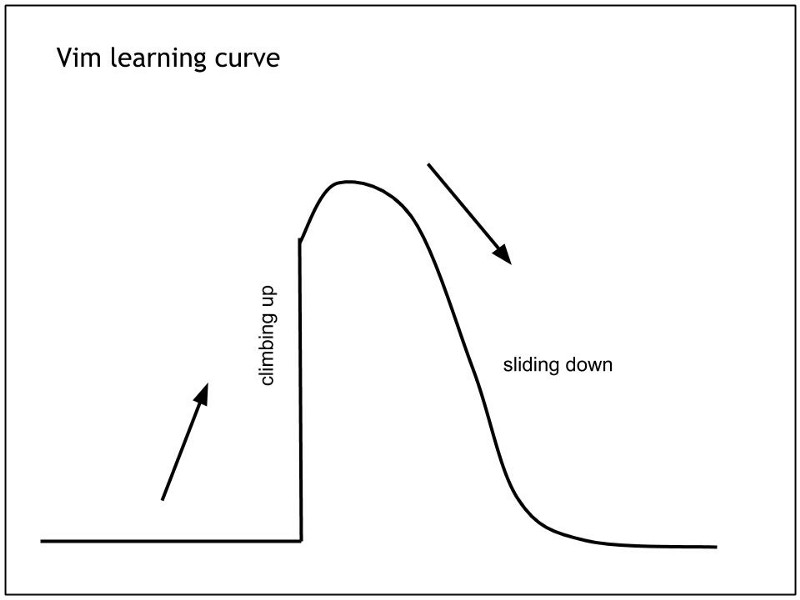
\includegraphics[width=\paperwidth,height=\paperheight]{images/learning-wall.jpeg}}
\begin{frame}
    \frametitle{Vim learning wall}
\end{frame}

\usebackgroundtemplate{}
\begin{frame}
    \frametitle{Where to find me}
    www.mauri.codes
    \begin{block}{Open Questions}
        Is every even number the sum of two primes?
    \end{block}
\end{frame}

\begin{frame}[fragile]
    \frametitle{Code example}
    \inputminted{js}{codes/example.js}
\end{frame}

\begin{frame}
    \frametitle{Second Slide}
\end{frame}

\end{document}

#if 0
Question for the audience:
* How many of you here uses Vim on there daily basis?
* How many of you have used Vim before?
* How many of you have heard of vim but haven't give it a try?

Start from basic stuff with learning wall and what vim is. Wall as a joke.
With vim you only use the keyboard. Which in the end will make your code editing
a lot faster.
You might be conserned about can vim do something that my current IDE can.
Probably answer is yes.
You will get rid of constant hand movement to your mouse and also to your arrow
keys.
You will keep learning new things about vim for many years to come. There is
quite often to better way to do things.
At the beginning editing might seem slow and clungy but over time your will get
better with practice.
To practise vim try to push yourself to learn new things and how to do things
better.
When you get rid of your mouse and keybindings come naturally to you, your
efficient as an editor will go up dramatically.
Show some keybindings in action what are worth it. Change in stuff parenhesis,
quetos etc.
Vim will consumer your time to learn and configure. After that payoff will be
worth it. Vim is hard because it's different. It's different because it's
better.
What modes vim has.
Go through some vim features like motions, dot, registers.
Go through some basic verbs and then text objects and motions on top of that.
Vim plugin system. Some plugins I have (fzf, ag, NerdTree, YouCompleteMe)
Change your escape key! Maybe this with some of my settings
Going through these should cover pretty basic vim usage and take some time too.
At the end Vim on different platforms (WSL for Windows).
Where to start with vim (vimtutor).
At the beginning don't copy anyones .vimrc file or download all plugins. Just
get started without any and modify things on your own. This things will get like
what you like them to be. Reading some other people blogs or vimrc files for
examples and add them to your own.
Add your own vimrc to version control or similar. Mine is in dropbox.
Maybe show something from my .vimrc.
Vim keybinding elsewhere (Vimium on Chrome, i3 window manager etc.)
#endif
